\subsubsection{Contexte technique}

J'étais autonome sur la partie technique du travail. En effet, mes collègues développeurs étaient tous en alternance ou stagiaires. Nous nous formions donc tous en même temps, en nous entraidant.

C'est un contexte classique en informatique, l'apprentissage technique se fait souvent seul grâce aux documentations en ligne des outils utilisés. C'est d'ailleurs comme cela que nous forme l'\epita.

L'école a conscience que le domaine de l'informatique évolue trop vite pour nous apprendre des outils techniques, et préfère nous apprendre des méthodes de travail et nous donner l'habitude d'avoir la curiosité d'aller chercher l'information.

\begin{figure}[H]
    \centering
    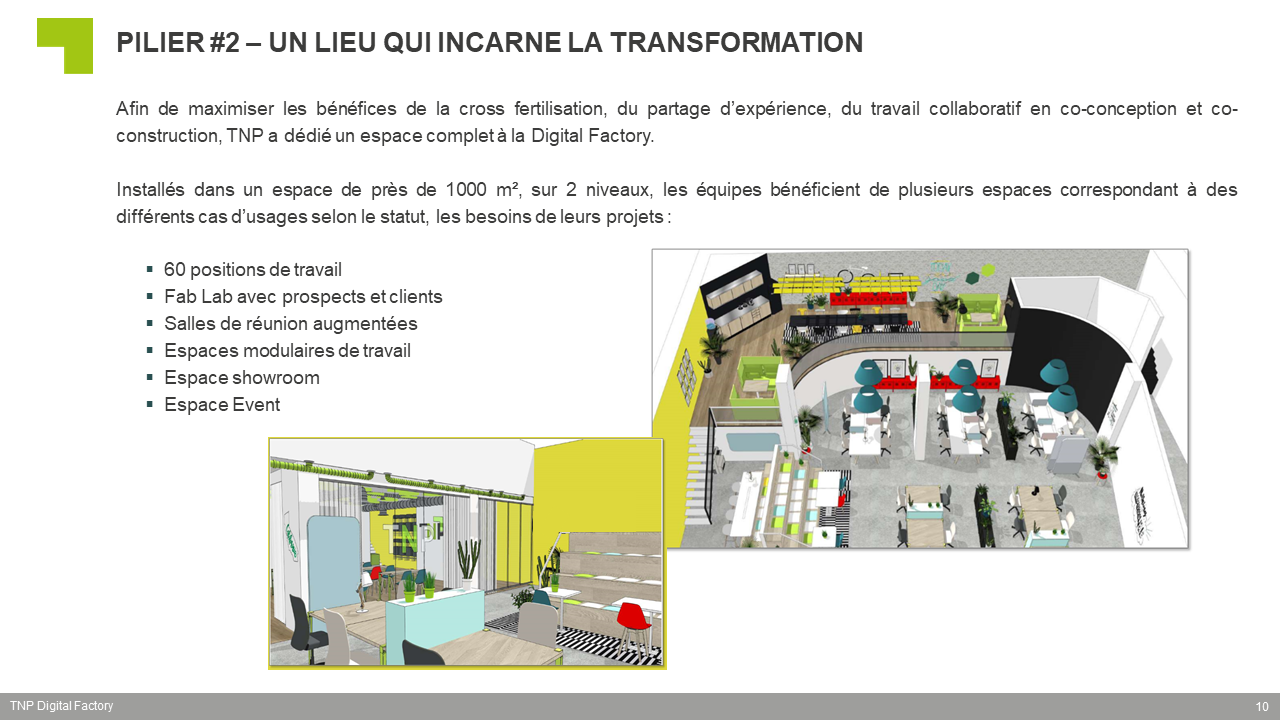
\includegraphics[width=1\linewidth]{img/digital_factory_lieu.png}
    \caption{Présentation des bureaux de la Digital Factory}
\end{figure}

\subsubsection{Contexte organisationnel et méthodes de travail}

La mission d'un ingénieur ne s'arrête cependant pas à l'aspect technique des choses. Il ne s'agit pas simplement d'exécuter des tâches.

\damien et \stefan nous ont aidés à comprendre le réel besoin du client. Ils assistaient aux réunions hebdomadaires avec le client, et pouvaient ensuite nous expliquer l'usage et les fonctionnalités recherchées par la \sncf. De plus, \stefan avait réfléchi en amont à la partie \gls{ux} du projet et visualisait donc encore mieux le résultat voulu par le client.

Aussi, l'expérience de \damien dans la gestion de projets numériques nous a aidés à faire les bons choix de technologies et outils pour répondre au besoin de manière pertinente.

\damien avait également une vision plus long terme du projet, puisqu'il avait déjà une idée des plannings et des évolutions futures souhaitées par client. Cela nous a aussi aidés à faire de meilleurs choix.

Finalement, j'ai effectué le travail de conception technique de manière autonome, mais avec l'aide de mes collègues et l'expertise des chefs.\\
Cependant, nous avons pu travailler avec \damien pour la réflexion en amont du projet, comme la compréhension réelle du besoin client, le choix des technologies et l'organisation des tâches du projet.